% !TEX root = ../../main.tex


\begin{figure}[!tbp]
	{\footnotesize\quad\texthv{\textbf{A.~ Hard\,breaks}}} \\
	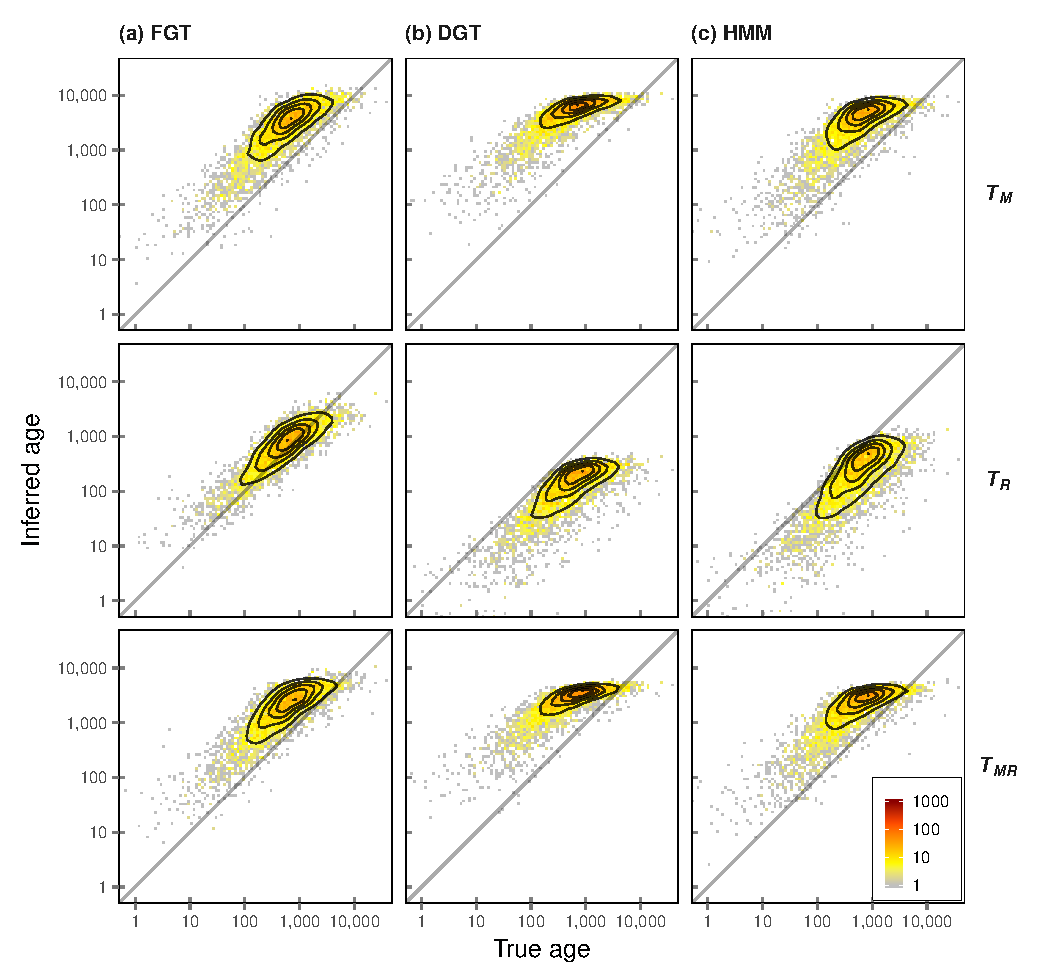
\includegraphics[width=\textwidth]{./img/ch5/vanilla_hard_breaks}
	\Caption{Comparison between inferred and true age}
	{Posterior mean age was estimated using the	\emph{hard\,breaks} method, Panel~\textbf{A}, and the \emph{soft\,breaks} method, Panel~\textbf{B} (see next page).
	Age is given in units of generations.
	The density of coinciding true and inferred age is indicated (colour-gradient).
	For visual aid, contours indicate regions of higher density, using bivariate  kernel density estimation.
	Analyses were conducted for \textbf{(a)}~\gls{fgt}, \textbf{(b)}~\gls{dgt}, and \textbf{(c)}~\gls{hmm}.
	In each, age was estimated under the \n{3} different clocks; \ie $\mathcal{T_{\!M}}$, $\mathcal{T_{\!R}}$, and $\mathcal{T_{\!M\!R}}$.
	In each comparison, results were generated on the same set of \n{5000} variants, which were pre-selected at random from alleles at $\leq5\%$~frequency.
	The number of discordant pairs was ${n_d = \num{1000}}$ in each comparison.}
	{fig:vanilla_plots:A}
\end{figure}

\begin{figure}[!tbp]
\ContinuedFloat
	{\footnotesize\quad\texthv{\textbf{B.~ Soft\,breaks}}} \\
	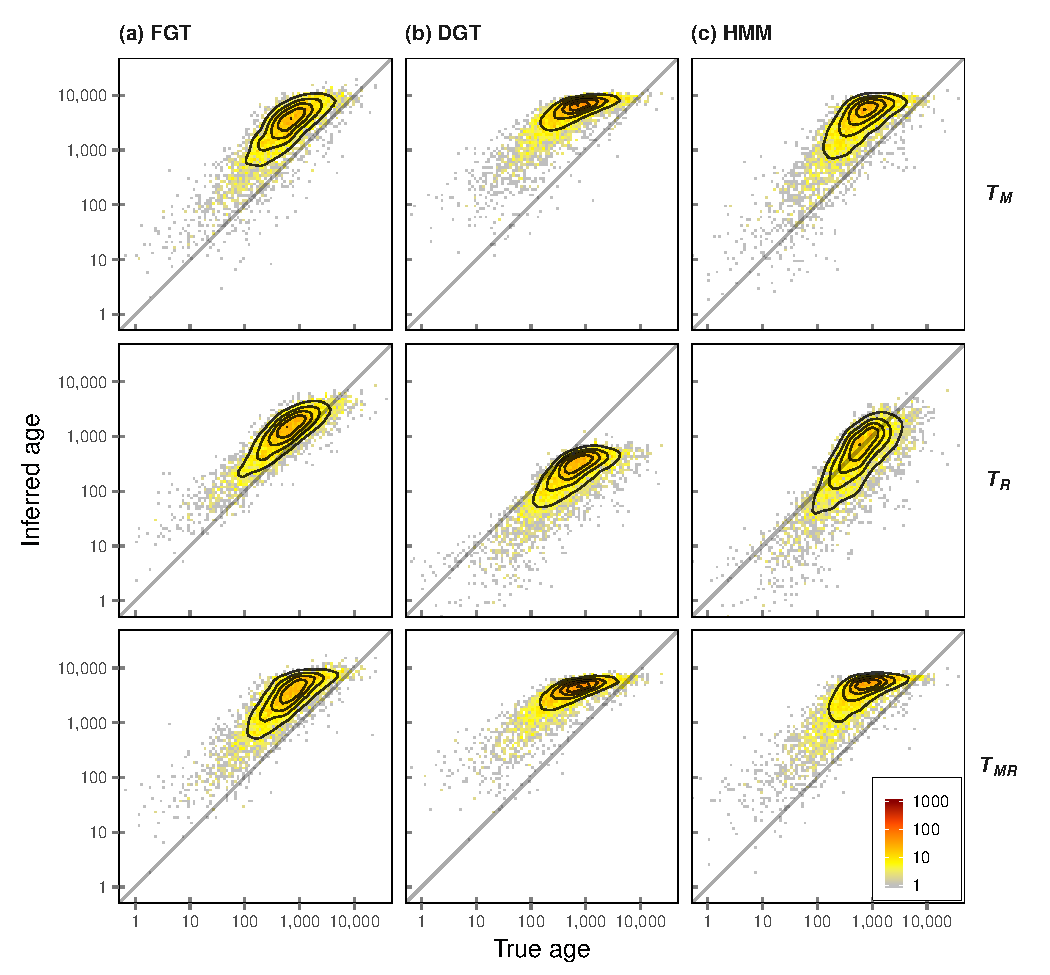
\includegraphics[width=\textwidth]{./img/ch5/vanilla_soft_breaks}
	%\Caption{Comparison between estimated and true age}
	\small
	\caption[]{Continued.}
	\label{fig:vanilla_plots:B}
\end{figure}
